\section{Context}
\label{design:context}

During the bootstrapping process, the bootware has to know certain things to be able do its job.
This information can be combined in one central object, which defines the nature of the current request: The context.
In this section we will take a closer look at this context object and its content.
How exactly the context is implemented is shown in \autoref{implementation:context}.

\begin{figure}[!htbp]
	\centering
	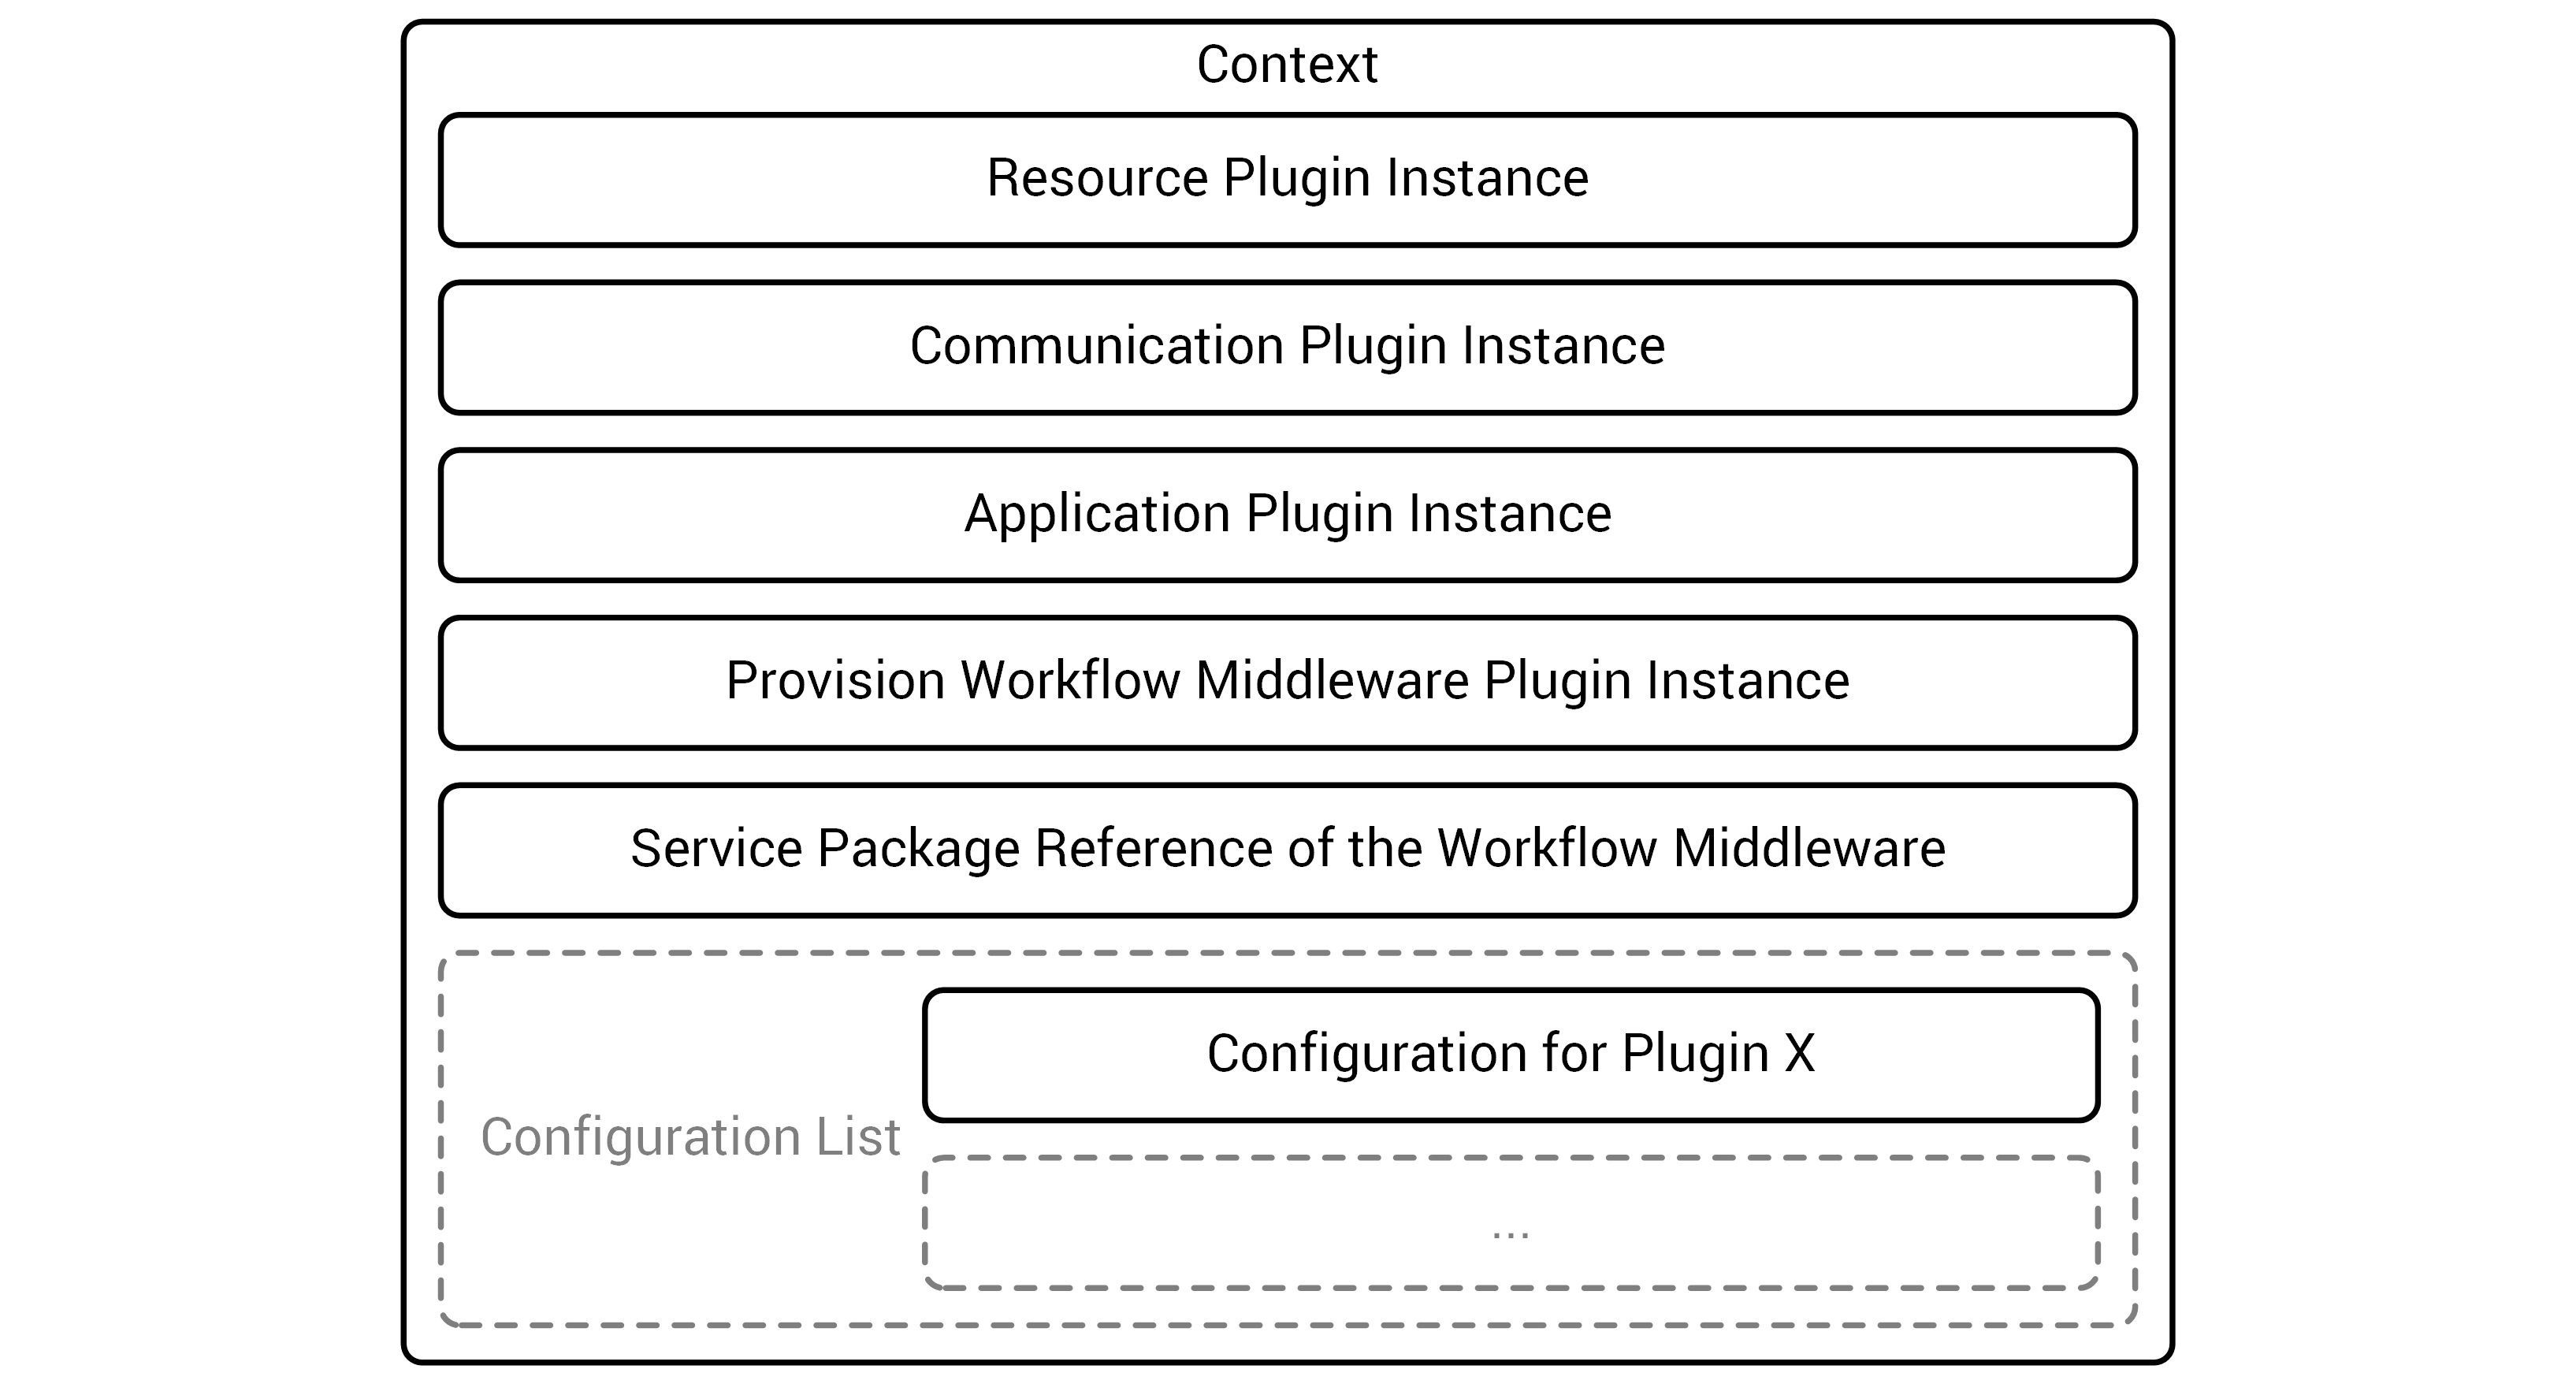
\includegraphics[resolution=600]{design/assets/context}
	\caption{Content of the context object.}
	\label{image:context}
\end{figure}

\autoref{image:context} shows the context object and its content.
As we can see in the upper half of \autoref{image:context}, it defines the plugin types to be used for the current request.
The infrastructure plugin type defines, which infrastructure plugin should be used to provision the requested infrastructure.
The connection plugin type selects how the bootware should connect to to this infrastructure.
The payload plugin type defines the payload that should be provisioned on this infrastrucre, which will be a provisioning engine in most cases.
Finally, the provisioning engine plugin type defines the plugin that should be used to call the provisioning engine.
It will use the middleware package referende, which is also defined in the context, as input to start the provisioning of the workflow middleware.
In the bottom half of \autoref{image:context} we can see that the context can also contain login credentials for different infrastructure providers (i.e. cloud providers).
These will be used by the infrastructure plugins to connect to a specific account at their provider.
In the future, the context might be extended to hold additional information, but for this thesis, this context will be sufficient.

Now that we have defined how the context will look like, we need to find a way to actually get it to the bootware.
There are a few things that we have to keep in mind when doing this.
First, these values have to be changeable by the user, so it doesn't make sense to hard-code them into the bootware.
Furthermore, the lifetime of the information carried in the context varies quite a bit.
The plugin types are only useful for one request execution and are likely to change from request to request, for example if the provisioning manager wants to provision multiple services with different provisioning engines.
Therefore, we must provide the plugin types on a per request basis.
Since we already decided that we'll be using web services as external communication method, we can send the context containing the plugin types with each request as part of the soap message body.

The cloud credentials on the other hand aren't likely to change between requests.
Additionally, we have other components calling the bootware who don't know (and maybe shouldn't know) anything about login credentials, for example the provisioning manager.
While this might change in the future, it would make sense to be able to set the login credentials once when starting the bootware, so that they don't have to be delivered with each request and so that other components, who don't know them, can still use the bootware.
It should however still be possible to override or update the login credentials at a later point.
Overriding would allow any request to temporarily use other login credentials if necessary.
Updating the login credentials at a later point could be useful, for example if the user accidentally provided the wrong credentials at the beginning.
Without this functionality, the whole bootware process could fail (even while provisioning the very last service) and would have to be started again from the beginning.
This could be avoided by providing the functionality to change login credentials even during the bootstrapping process.

For setting the login credentials at the beginning and for updating them later during the process, a \textit{setCredentials} method will be added to the bootware web service.
The credentials set by this method will be treated as the default credentials by the Bootware.
If no other credentials are provided, these will be used during the process.
If however a request is send with a context that also contains login credentials, these credentials will override already existing default credentials temporarily for this request.
This behavior could also be extended to other parts of the context in future, if necessary.
